\subsection{Der globale Anwendungszustand}
Die Struktur des Quelletext wird durch die Verwendung von \emph{Redux} geprägt. Innerhalb der Datei \lstinline|reducers/rootReducer.ts| ist die Schnittstellendefinition \lstinline|IApplicationState| enthalten, welche den Aufbau des \emph{Redux-Store} des FreeDesign-Editors beschreibt. Die Schnittstelle enthält Eigenschaften, die den globalen Zustand in Unterbereiche aufteilt (Abbildung \ref{fig:IApplicationState}). Der Aufbau dieser Bereiche sind durch weitere Schnittstellendefinitionen beschrieben, die innerhalb der Typescript-Dateien im Ordners \lstinline|stores| implementiert sind. 
Im Anhang ist die Tabelle T1\_Redux-State.pdf enthalten, welche die Aufgaben der Unterbereiche einordnet. 


\begin{figure}[H]
    \centering
    \caption{Struktur der Schnittstelle \lstinline|IApplicationState| welche den \emph{Redux-State} des Freedesign-Editors beschreibt.}
    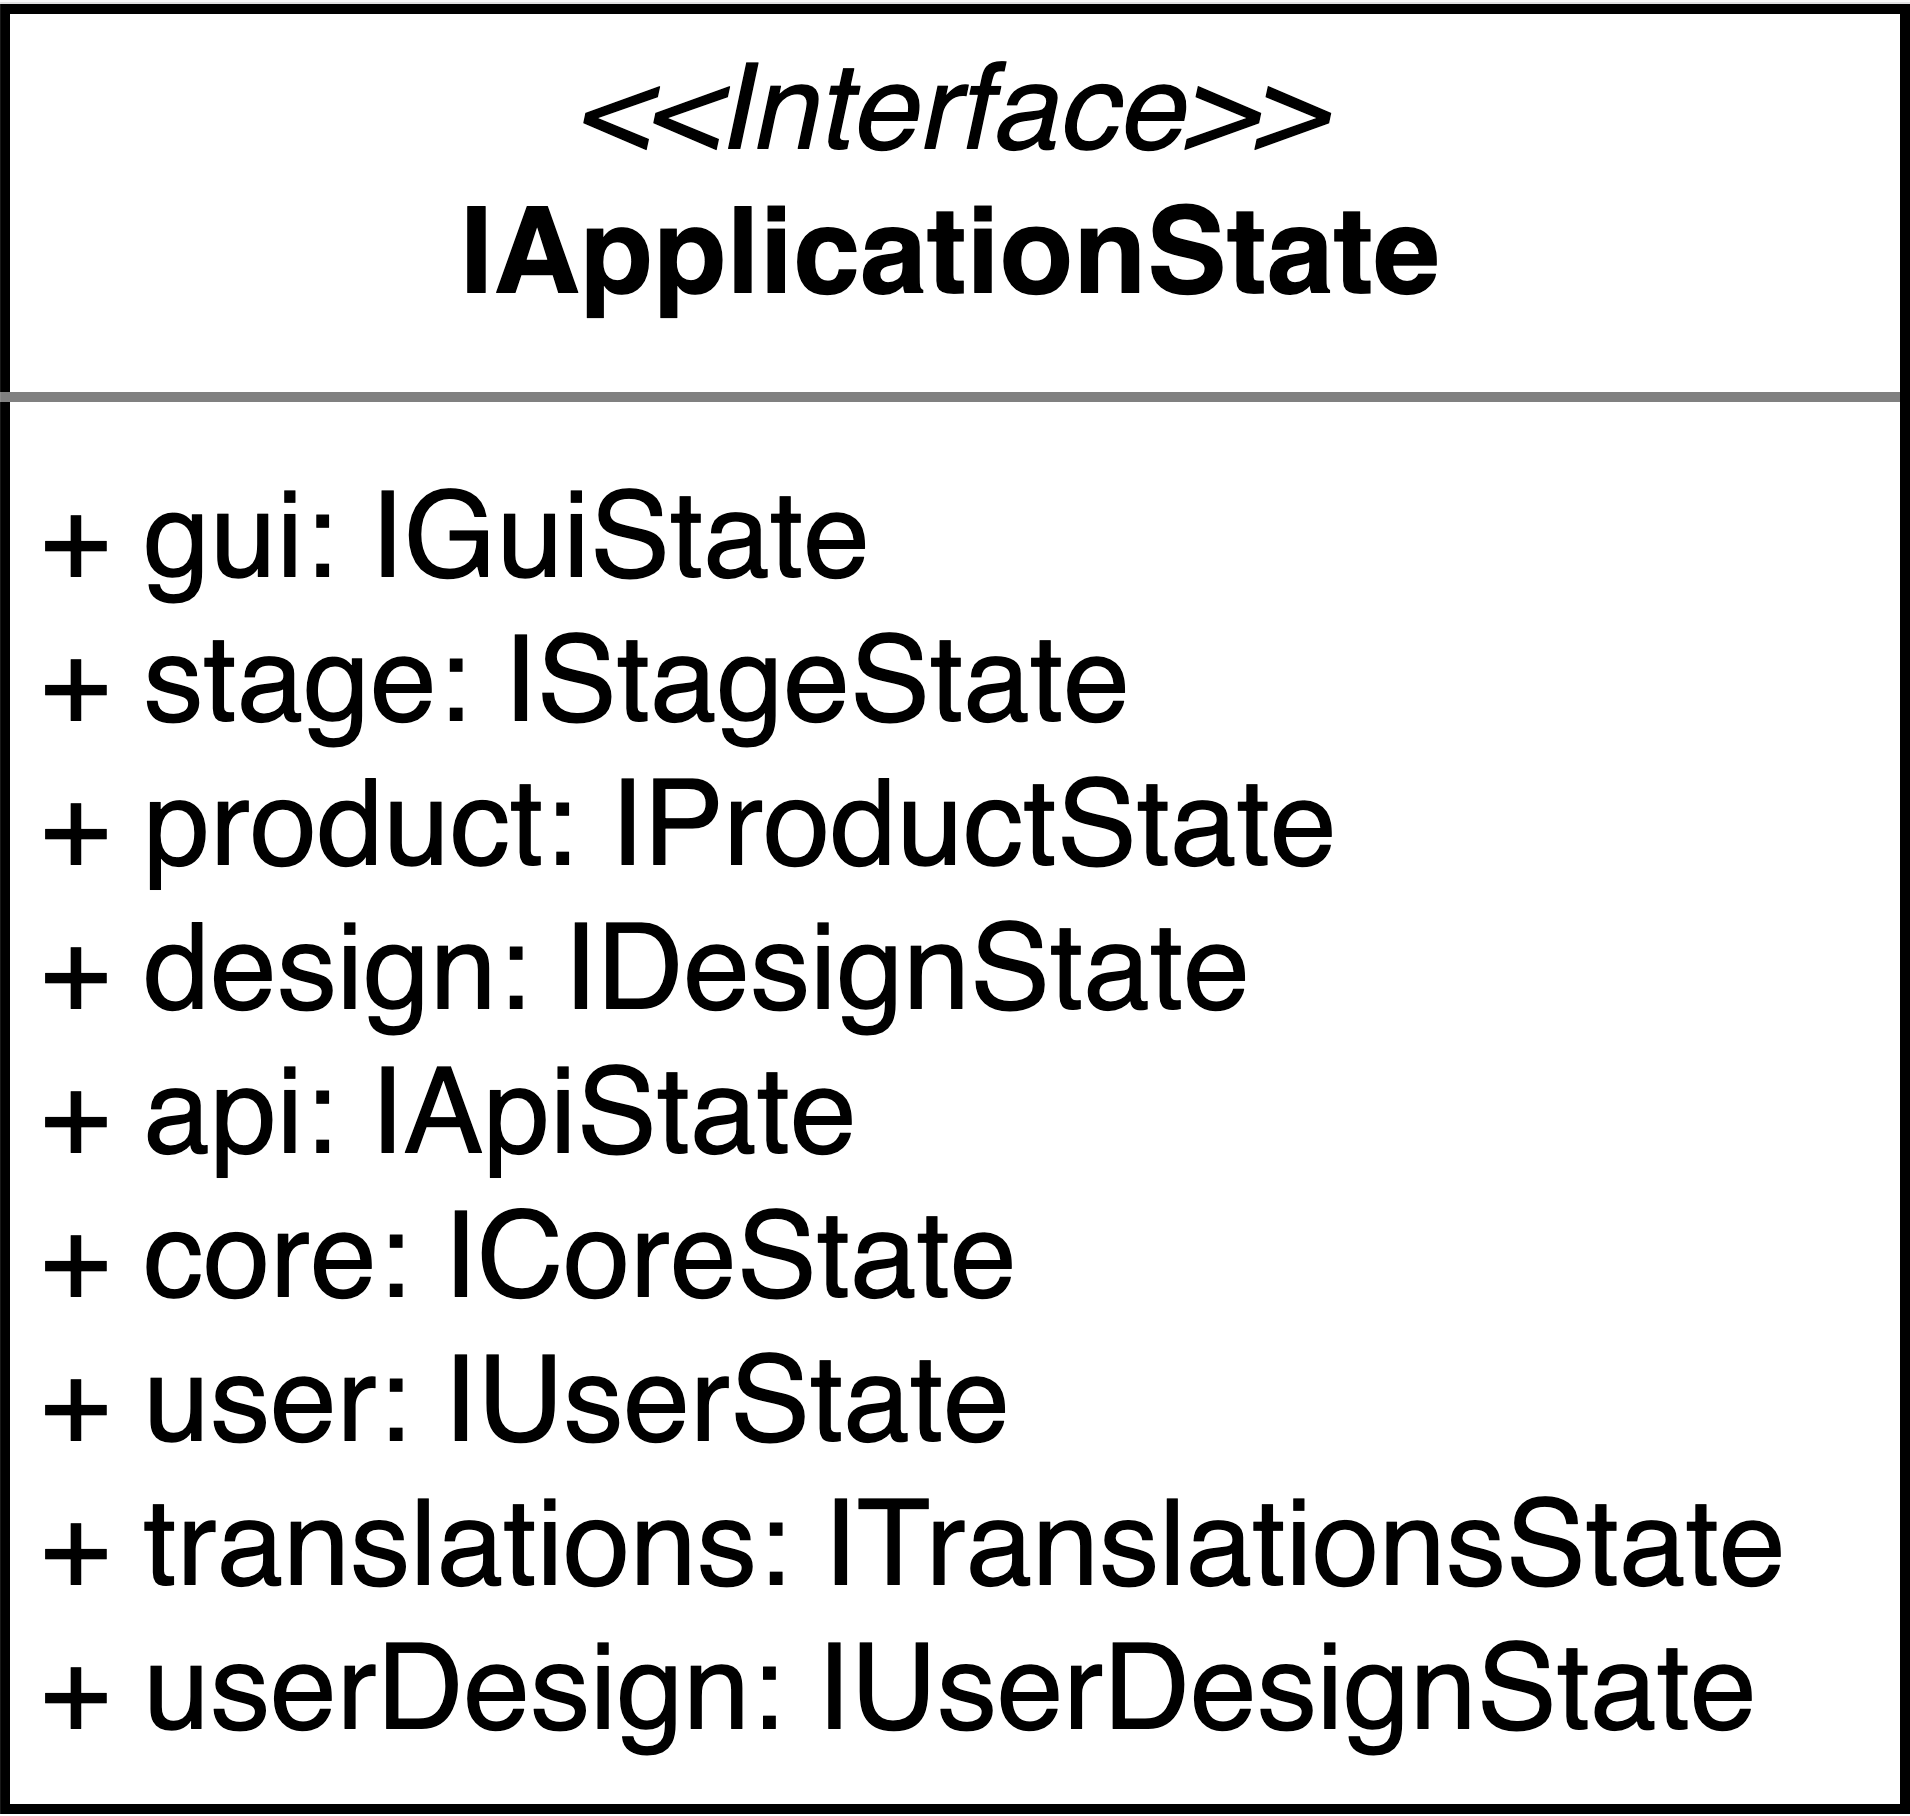
\includegraphics[width=.3\textwidth]{diagrams/Ist-Architektur/IApplicationState.png}
    \label{fig:IApplicationState}
\end{figure}


Im Anhang ist die Zip-Datei hinterlegt D1\_Redux.zip welche die Diagramme der Analyse der Redux-Struktur enthält.
Die Datei enthält folgende drei Ordner:  
\begin{itemize}
    \item Der Ordner \lstinline|stores| enthält Diagramme, die die Abhängigkeiten der Typescript-Dateien unter \lstinline|stores| aufzeigen.
    \item Der Ordner \lstinline|actions| enthält Diagramme, die die Abhängigkeiten der Typescript-Dateien unter \lstinline|actions| aufzeigen.
    \item Der Ordner \lstinline|reducers| enthält Diagramme, die die Abhängigkeiten der Typescript-Dateien unter \lstinline|reducers| aufzeigen. 
    \item Der Ordner \lstinline|containers| enthält Diagramme, die die Beziehung zwischen dem Order \lstinline|containers| und Redux-Ordner \lstinline|stores|, \lstinline|actions| und \lstinline|reducers| aufzeigen.
\end{itemize}
Alle Diagramme innerhalb der Ordner wurden mit dem Werkzeug \emph{Madge} erzeugt.
Die Zip-Datei enthält weiterhin das Diagram \lstinline|redux.html| welches mit dem Werkzeug \emph{dependency-cruiser} erzeugt wurde und die funktionalen Abhängigkeiten zwischen den vier Ordnern darstellt.

Basierend auf den Diagrammen wurde Abbildung \ref{fig:Redux} erstellt welches einen Überblick der Abhängigkeiten darstellt. Die Färbung der Beziehungspfeile dient Übersichtlichkeit des Diagrams und haben keine inhaltliche Aussage.

Die \emph{Container}-Komponenten im Ordner \lstinline|containers| greifen auf die Schnittstellendefinition innerhalb des Ordners \lstinline|stores| zu, sowie auf die Schnittstelle \lstinline|IApplicationState|. 
Außerdem rufen sie \emph{Redux-Actions} aus dem Ordner \lstinline|actions| auf.

Durch die Implementation von \emph{Redux-Actions} welche andere \emph{Redux-Actions} aufrufen, bestehen zwischen einigen  Actions Abhängigkeiten.  

Jede \emph{Redux-Action} ist von einem spezifischen Typ, welche innerhalb des Ordners \lstinline|actions/types| definiert sind. Auf der Basis des Typ erzeugen die \emph{Redux-Reducer} einen neuen \emph{Redux-State}.

\begin{figure}[H]
    \centering
    \caption{Darstellung der Zugriffe zwischen den Ordnern \lstinline|store|, \lstinline|actions| und \lstinline|reducers|.}
    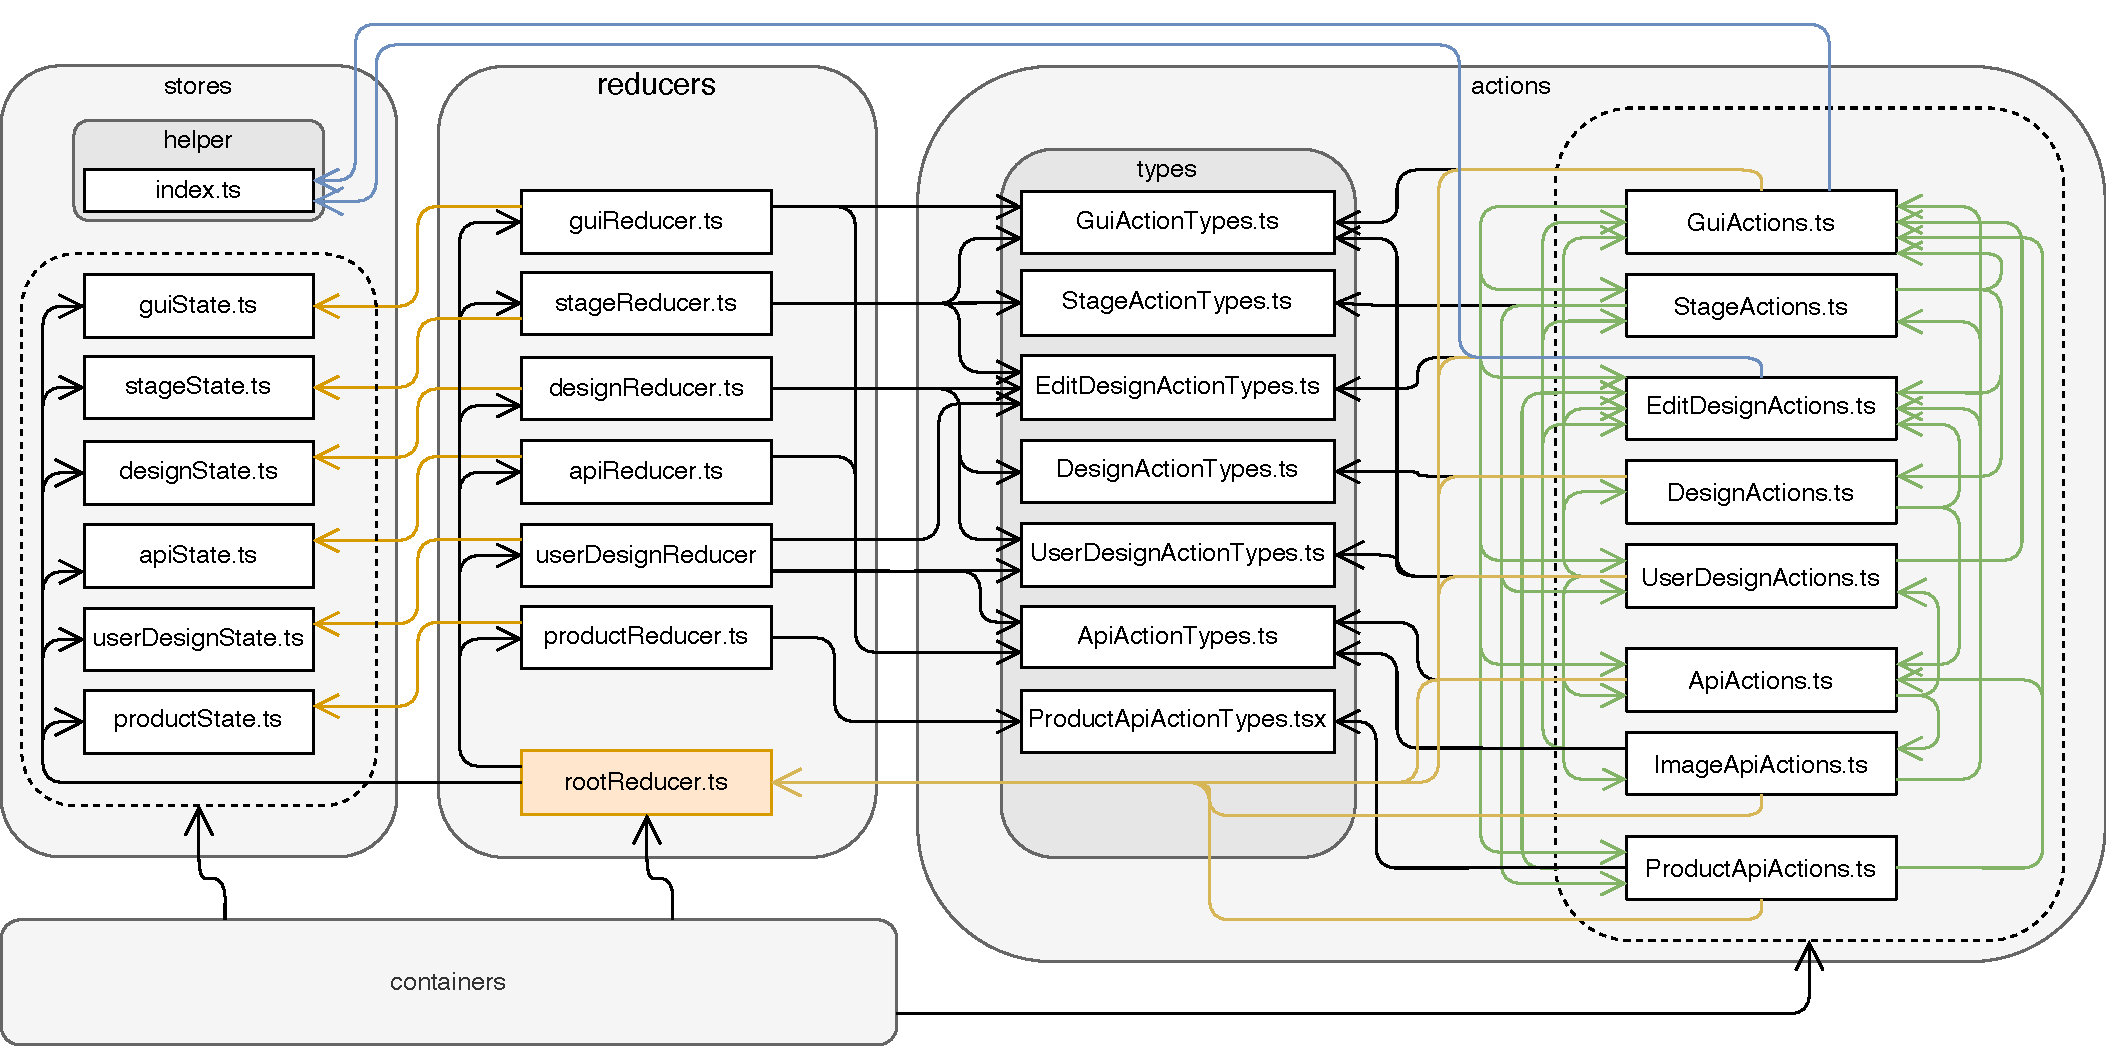
\includegraphics[width=1\textwidth]{diagrams/Ist-Architektur/Redux.pdf}
    \label{fig:Redux}
\end{figure}



